%
\section{\color{red}Introduction\label{ptInt}}

%
\section{Methods \label{meth}}

\subsection{Model}

%
%Below I present the three-parameter Pella-Tomlinson (PT) family, which has a 
The three-parameter Pella-Tomlinson (PT) family has a convenient form that includes, among
others \cite{fox_jr_exponential_1970,rankin_alternative_2015}, the
logistic production function as a special case. %Under logistic production to form the Schaefer model. The 
PT production function is parameterized so that $\bm{\theta} = [r, K, \gamma]$
and the family takes the following form,
%Pella Tomlinson
\begin{align}
P_{p}(B; [r, K, \gamma]) = \frac{r B}{\gamma-1} \left(1-\left(\frac{B}{K}\right)^{(\gamma-1)}\right). \label{pt}
\end{align}

%\clearpage

%
\begin{wrapfigure}{r}{0.45\textwidth} %[17]{r}[0pt]{0pt}%
%\begin{figure}[h!]
\vspace{-1cm}
%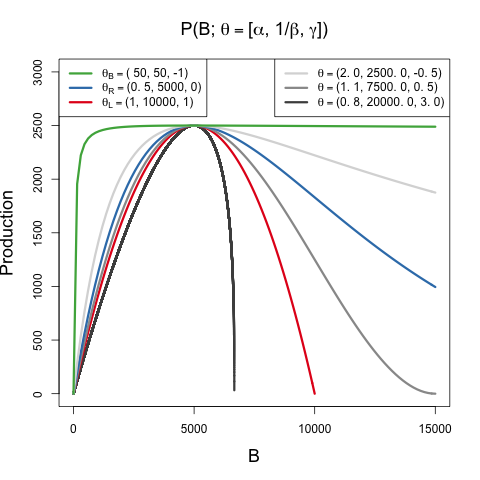
\includegraphics[width=0.5\textwidth]{plots/derisoSrr.png}
%\begin{minipage}[h!]{0.64\textwidth}
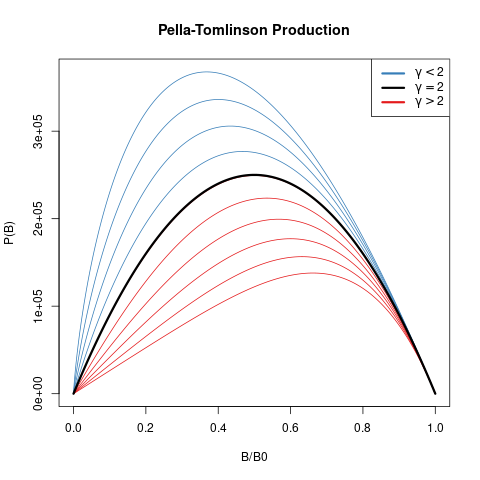
\includegraphics[width=0.49\textwidth]{../ptNew/g4PT.png}
%\end{minipage}
%\begin{minipage}[h!]{0.3\textwidth}
\vspace{-1cm}
%\hspace*{-1cm}
\caption{
%\onehalfspacing
The Pella-Tomlinson production function plotted across a variety of parameter
values. The special cases of Logistic production is shown in black, and the
left-leaning and right-leaning regimes are shown in blue and red respectively.
}
\label{SrrPT}
%\end{minipage}
\end{wrapfigure}
%\end{figure}

%
$\gamma$ is a parameter which breaks PT out of the restrictive symmetry of the
logistic curve. In general $\gamma\in(1, \infty)$, with the logistic model
appearing in the special case of $\gamma=2$, and the Fox model appearing as
a limiting case as $\gamma\to1$.
%In the special case of $\gamma=2~$ Eq (\ref{pt}) 
%collapses back to the logistic curve, however in general $\gamma\in(1, \infty)$.
%
%The parameters $r$ and $K$ maintain the same interpretation as 
%they do in the logistic production function. In Figure (\ref{SrrPT}) PT recruitment 
%is shown for a range of parameter values so as to demonstrate the various 
%recruitment shapes that can be achieved by PT recruitment.  
%reproductivei (biomass accumulation)
The parameter $r$ controls the maximum per-capita growth rate of the population
in the absence of competition for resources (i.e. the slope of production
function at the origin). $K$ is the so called "carrying capacity" of the
population. In this context the carrying capacity can be formally stated as
steady state biomass in the absence of fishing \mbox{(i.e. $\bar B(0)=K$).}
%
In Figure (\ref{SrrPT}) PT production is shown for a range of parameter values
so as to demonstrate the various productivity shapes that can be achieved under
PT.

%
While the form of the PT curve produces some limitations \cite{fletcher_restructuring_1978}, %{(\color{red}cite)}, 
importantly the % how $\gamma$ appears in PT still produces some limitations to the form of the production function 
introduction of a third parameter allows enough flexibility to fully describe
the space of reference points used in management. To see this, the reference
points are analytically derived for the PT model below. % in the following section.

%
\subsection{Reference Points}\label{ptRef}
%
With $B(t)$ representing biomass at time $t$, under PT production, the
dynamics of biomass are defined by the following ODE,

\begin{equation}
\frac{dB}{dt} = \frac{r B}{\gamma-1} \left(1-\left(\frac{B}{K}\right)^{\gamma-1}\right) - FB. \label{dBdtPT}
\end{equation}

An expression for the equilibrium biomass is attained by setting Eq (\ref{dBdtPT})
equal to zero, and rearranging the resulting equation to solve for $B$.
Thinking of the result as a function of $F$ gives,
%When thought of as a 
%function of $F$ the following expression emerges,
%{\color{red}Under Pella-Tomlinson SRR the equilibrium biomass can be written,}
\begin{align}
\bar B(F) = K\left(1-\frac{F(\gamma-1)}{r}\right)^{\frac{1}{(\gamma-1)}}. \label{BbarPT}
\end{align}

%By definition $B_0=K$. Alternatively, Setting $F=0$ in Eq(\ref{Beq}) makes it convenient to notice that $\bar B(0)=K$ to arrive at the same result
At this point it is convenient to notice that $\bar B(0)=K$. The expression for
$B^*$ is given by evaluating Eq (\ref{BbarPT}) at $F^*$.
%
To get an expression for $F^*$, the equilibrium yield is maximized with respect to $F$,
\begin{equation}
F^* = \argmax_F F\bar B(F).
\end{equation}
%
In the case of PT production this maximization can be done analytically, %. In this case maximization can proceed 
by differentiating the equilibrium yield with respect to $F$ as follows,
%
\begin{align}
\frac{d \bar{Y}}{dF} &= \bar B(F) + F \frac{d \bar B}{dF} \label{FderivPT}\\
%\frac{d \bar B}{dF} &= -\frac{K}{\gamma-1}\left(\frac{\gamma-1}{r}\right)^{\frac{1}{\gamma-1}}F^{\frac{1}{\gamma-1}-1}\\
\frac{d \bar B}{dF} &= -\frac{K}{r}\left(1-\frac{F(\gamma-1)}{r}\right)^{\frac{1}{\gamma-1}-1}\label{dBdFPT}.
\end{align}

%{\color{red}
Setting Eq (\ref{FderivPT}) equal to 0, substituting $\bar B(F)$ and
$\frac{d \bar B}{dF}$ by Equations (\ref{BbarPT}) and (\ref{dBdFPT}) respectively,
and solving for $F$ produces the following expression for the fishing
rate required to produce MSY, %{\color{red}Below any quantity evaluated at MSY shall be decorated with $~^*$.}
%
\begin{align}
F^* = \frac{r}{\gamma}%-1} \left(\frac{\gamma-1}{\gamma}\right)^{\gamma-1}. \label{Fmsy}
\end{align}

%
Plugging the above expression for $F^*$ back into Eq (\ref{BbarPT}) gives the
following expression for biomass at MSY,
\begin{align}
B^* = K\left(\frac{1}{\gamma}\right)^{\frac{1}{\gamma-1}} \label{BmsyPT}. %\left(1-\left(\frac{\gamma-1}{\gamma}\right)\right) \label{Bmsy}.
\end{align}

%
The above derived expressions for $\bar B(0)$, $B^*$, and $F^*$ can then be used to
build a specific analytical form for the biological reference points in terms of only
productivity parameters.
%%
%By substituting the expressions given above for $B_0$, $B^*$, and $F^*$ into 
%Eq(\ref{xizetaSimple}), $\xi$ and $\zeta$ can take a specific analytical form 
%in terms of the biological model parameters. 
%%given by substituting the expressions given in Eq(\ref{Fmsy}) 
%%and Eq(\ref{Bmsy}) in Eq(\ref{xizetaSimple}).
%%Eq(\ref{xizetaSimple}) can then take a specific analytical form in terms of the 
%  %an expression for $\xi$ and $\zeta$ can be found in terms of model parameters.  
\begin{align}\label{ptRP}
&F^* = \frac{r}{\gamma}
&\frac{B^*}{\bar B(0)} = \left(\frac{1}{\gamma}\right)^{\frac{1}{\gamma-1}}
\end{align}

%
\subsection{Simulation}

%speaking it is not possible to analytically invert this  
Generating simulated indices of abundance from the PT model requires
inverting the relationship between $\left(F^*, \frac{B^*}{\bar B(0)}\right)$, and
$(r, \gamma)$. It is not generally possible to analytically invert this
relationship for many three-parameter production functions \cite{punt_extending_2019, schnute_analytical_1998}. %{(\color{red}cite Derizo paper)}. 
Most three-parameter production functions lead to RPs that require expensive
numerical methods to invert; more over the numerical inversion procedure can %is 
often be unstable. That said, for the case of PT this relationship is
analytically invertible, and leads to the following relationship
%
\begin{align}
&r = \gamma F^*
&\gamma = \frac{W\left(\frac{B^*}{\bar B(0)}\log\left(\frac{B^*}{\bar B(0)}\right)\right)}{\log\left(\frac{B^*}{\bar B(0)}\right)}. \label{gammaOfB}
\end{align}
%
%Above $W_0$ is the principal branch of the Lambert product logarithm function. 
%Above $W_{-1}$ is the lower branch of the Lambert product logarithm function. 
Above $W$ is the Lambert product logarithm function. More details about this
derivation, and the Lambert product logarithm, are given in \mbox{Appendix (\ref{lambApp}).}

%
Using Eq. (\ref{gammaOfB}) to obtain production parameters, a PT production model
can be fully defined for any combination of the RPs $F^*$ and $\frac{B^*}{\bar B(0)}$.
Since $K$ does not enter the RP calculation its value is fixed arbitrarily at 10000.

%
%\begin{itemize}
%       \item introduce metamodeling idea
%       %\item some design details
%\end{itemize}
%

%$\sigma$ is fixed at the relatively small value of 0.01 to focus specifically on the
%behavior of population parameters.

%
%The index residual standard deviation, $\sigma$, is fixed to the relatively 
%small value of 0.01 to focus specifically on the behavior of productivity 
%parameters.

Indices of abundance are simulated from the three-parameter PT production model
broadly over the space of $F^*$ and $\frac{B^*}{\bar B(0)}$ via a space filling
design as described in Section (\ref{lhs}). A small amount of residual variation,
$\sigma=0.01$, is added to the simulated index, and these data are then fit with a
Schaefer model, at various degrees of misspecification, so as to observe the
effect of productivity model misspecification upon RP inference.

%
\subsection{Design}

%
Letting $\mathcal{F}$ and $\mathcal{B}$ be regular grids, of size $n=100$, on
\mbox{$F^*\in(0.1, 0.7)$} and \mbox{$\frac{B^*}{B_0}\in(0.2, 0.6)$}
respectively, a LHS design of size 100 is collected among the cells produced by
$\mathcal{F}\times\mathcal{B}$. 

%
Each of the sampled LHS design locations represent a unique PT model with the
sampled RP values. Since the relationship mapping RPs analytically to productivity
parameters can be found for the PT model, LHS designs the the PT model are 
computed directly in RP space and Eq. (\ref{gammaOfB}) is used to map the
sampled RP design locations to PT productivity parameters.

%
\subsection{Gaussian Process Metamodel}
%

%
At its core, a metamodel is simply a model of some mapping of inputs to outputs
(the mapping itself is typically defined by a computer model). By modeling the
mapping with a statistical model (that explicitly defines the relevant features of the
mapping) a metamodel defines a specific ontology for the mapping.
%representation of an ontology of the modeled mapping. %the mapping %that can be seen to form
%By modeling the mapping as a statistical model, and 
By simulating examples of the mapping, the inferential infrastructure of the
statistical model is used to empirically learn an effective emulation of the
mapping within the ontology defined by the statistical model. %, based on simulated examples of the mapping. 
The predictive infrastructure of the statistical model is then useful as an
approximate abstraction of the system itself to better understand the system
through further data collection, cheap approximation of the mapping, and/or study
of the mapping itself.

%\begin{itemize}
%\item Goal of metamodel
%\begin{itemize}
%       \item General
%       \item Metamodel can be a mathematical relation or algorithm representing input and output relations.
%       \item Metamodeling typically involves studying the output and input relationships 
%               and then fitting right metamodels to represent that behavior. 
%       \item As an approximation of a higher-fidelity model for use when reducing time, cost, or computational effort is necessary
%       \item Meta-models are closely related to ontologies. 
%               Both are often used to describe and analyze the relations between concepts
%       \item an ontology is a way of showing the properties of a subject area and how they are related, 
%               by defining a set of concepts and categories that represent the subject. 
%       \item A valid metamodel is an ontology, but not all ontologies are modeled explicitly as metamodels
%       \item An explicit ontology.
%\end{itemize}
%\item what do GPs do
%\begin{itemize}
%       \item A GP is a stochastic process generalizing the multivariate normal distribution
%       to an infinite dimensional analog. GPs are often specified primarily through the
%       choice of a covariance (or correlation) function which defines the relationship
%       between locations in an index set. Typically the index set is spatial for GPs,
%       with points closely related in the index set resulting in correlated effects in
%       the model. In this setting the model is over the space of reference points.
%       A GP model implies an $n$ dimensional multivariate normal distribution on the
%       observations of the model with a correlated error structure defined by the
%       modeled covariance function.
%\end{itemize}
%\item explain math. application.
%\end{itemize}

%
In this setting, the aim of metamodeling is to study how well RPs are inferred
when typical two-parameter models of productivity (Logistic and BH) are
misspecified for populations that are actually driven by more complicated
dynamics. The simulation design, $\bm{X}$, provides a sample of different
population dynamics that are driven by three-parameter production functions
broadly in RP space. By simulating index of abundance data from the three
parameter model, and fitting those data with the two-parameter production model, we %one can 
observe particular instances of how well RPs are inferred at the given
misspecification of the two-parameter model relative to the true three-parameter
production model. By gathering all of the simulated instances of how RPs are
inferred (under the two-parameter model), %under misspecified two-parameter models
we form a set of example mappings to train a metamodel which represents the
mapping of true RPs (under the three-parameter model) to estimates of RPs under the
misspecified two-parameter production model. The metamodel is essentially a surrogate
for inference under the misspecified two-parameter production model that
controls for the specific degree of model misspecification.
%the way in whthe nature of  
%specific misspecification of RP. 
%to how poorly the
%when two-parameter production models infer RPs relative to how poorly the %the degree of RP 
%model is specification. %more generally.

%
A flexible GP model is assumed for the structure of the metamodel to describe the mapping
of RPs under misspecified two-parameter models of productivity. A GP is a
stochastic process generalizing the multivariate normal distribution
to an infinite dimensional analog. GP models are often specified primarily
through the choice of a covariance (or correlation) function which defines the
relationship between locations in the input space. %an index set. Typically the index set is spatial for GPs,
%with points closely related in the index set resulting in correlated effects in
%the model. 
Typically correlation functions are specified so that points closely related in
space result in correlated effects in the model. In this setting the inputs to
the GP metamodel are the space of reference points which define the simulated
three-parameter production models.
%The GP model then implies a multivariate normal response distribution on the
%observations of the model with a correlated error structure defined by the
%modeled covariance function.

%
While index of abundance data are generated from three-parameter models, at each
design location of the simulation, fitting the restricted two-parameter model
results in a maximum likelihood estimate (MLE; and associated estimation
uncertainty) of each of the productivity parameters
{\color{red}
(i.e. Schaefer:[$log(r)$, $log(K)$], BH:[$log(\alpha)$, $log(\beta)$]).
}
% as well as estimation uncertainty (via the inverted Fisher information).
%At each design location of the simulation, fitting the restricted two-parameter
%model results in a MLE of each of the productivity parameters
%(i.e. Schaefer:[$log(r)$, $log(K)$], BH:[$log(\alpha)$, $log(\beta)$]).
To simplify the specification of the metamodel, let $\textbf{y}$ be a vector
collecting the fitted MLEs for one of the productivity parameters, and let
$\bm{\omega}$ be a vector of estimates of the estimator variances (via the
inverted Fisher information) at each $\textbf{y}$.
%
Each of the fitted productivity parameter estimates are then modeled using
independent instances of the following GP metamodel. %in Eq (\ref{GPModel}). 
\begin{align} \label{GPModel}
        \textbf{y} &= \beta_0 + \bm{X}\bm{\beta} + \bm{v} + \bm{\epsilon} \nonumber \\
        \bm{v} &\sim N_n(\bm{0}, \tau^2 \bm{R_{\ell}}) \\
        \bm{\epsilon} &\sim N_n(\bm{0}, \bm{\omega}'\bm{I}) \nonumber
\end{align}
%%
%Let $\textbf{y}$ be a vector collecting the fitted log productivity parameter MLEs under 
%the restricted two-parameter production models. Furthermore, let $\bm{\omega}$ 
%be a vector of the MLE standard error estimates, on the variance scale (via the inverted Fisher 
%information of the production model log likelihood).  
%


%, as derived above,
$\bm{X}$ is the $n$ x 2 LHS design matrix of RPs for each simulated %respective 
three-parameter data generating model as described in Section (\ref{desRef}).
%The GP residual variation
$\epsilon$ models independent normally distributed error, which provides an
ideal mechanism for propagating uncertainty from inference in the simulation
step into the metamodel. By matching each $\text{y}_i$ with an observed $\omega_i$
variance term, $\epsilon$ serves to down weight the influence of each $\text{y}_i$
in proportion to the inferred production model sampling distribution
uncertainty. This has the effect of smoothing the GP model in a way similar to
the nugget effect \cite{gramacy_cases_2012}, although the application
here models this effect heterogeneously.

%Above $\bm{v}$ is a vector of Gaussian process effects
The term, $\bm{v}$, contains spatially correlated GP effects. The correlation
matrix, $\bm{R_{\ell}}$ describes how RPs close together in the simulation design
are more correlated than those that are far away. This spatial effect is modeled
with a squared exponential correlation function,
%
\begin{align}   \label{corModel}
R(\bm{x}, \bm{\tilde x}) &= \exp\left( \sum_{i=1}^2 \frac{-(x_{i}-\tilde x_{i})^2}{2\ell_j^2} \right).
\end{align}

$R$ has an anisotropic separable form which allows for differing length scales,
$\ell_1$ and $\ell_2$, in the different RP axes. The flexibility to model
correlations separately in the different RP axes is key due to the differences
in the extent of the RP domains marginally.
%$\ell_1$ and $\ell_2$ model the length scales for $F^*$ and 
%$\frac{B^*}{\bar B(0)}$
%respectively. 
The metamodel parameters $\beta_0$, $\bm{\beta}$, $\tau^2$,
$\ell_1$ and $\ell_2$ are fit via MLE against the observations $\textbf{y}$, $\bm{X}$,
and $\bm{\omega}$ from simulation fits.

%
Fitting the metamodel allows for a full predictive description of inference
under the misspecified restricted models.
Predictive estimates are obtained via kriging \cite{cressie_statistics_2015} %{(\color{red}cite)}. 
%over intermediate values over RP space. 
%with $\hat~$ decorate any quantity that is derived for metamodel interpolation.
%{\color{red}Let $\tilde~$ decorate any quantity that is derived 
%under the metamodel prediction.}
\begin{equation} %k(x) a n−vector with kν,j (x) = K(x, xj ), for all xj ∈ X
        \hat y(\textbf{x}) = \beta_0 + \textbf{x}\bm{\beta} + \textbf{r(x)}'\bm{R}^{-1}_{\bm{\ell}}\Big(\textbf{y}-\big(\beta_0+\bm{X}\bm{\beta}\big)\Big)
\end{equation}

%
$\hat y(\textbf{x})$ is the predicted value of the modeled productivity parameter
MLE under the two-parameter production model, when the index of abundance %the metamodel at the 
is generated from the three-parameter production model at RP location $\textbf{x}$.
$\textbf{r(x)}$ is a vector-valued function of correlation function evaluations for the
predictive location $\textbf{x}$ against all observations in $\bm{X}$
(i.e. $\textbf{r(x)}=\bm{R}(\textbf{x}, \bm{x}_i)~\forall~\bm{x}_i\in\bm{X}$).

%
{\color{red}
While metamodeling occurs on the inferred productivity parameters of the
restricted production model, the metamodel can also be used to build
estimates of major biological RPs. For the BH model the relevant
transformations for relating productivity parameters with RPs are given in
Eqs. (\ref{BratS}, \ref{FmsyS}) with $\gamma$ fixed to -1; for the Schaefer
model $\hat B^*=\frac{\hat K}{2}$ and $\hat F^*=\frac{\hat r}{2}$.
%reference points.
%%estimate of two productivity parameters under the restricted production model. Each of the fitted productivity parameter
%%estimates are then modeled using independent instances of the following model in Eq (28).
%
Applying the metamodel predictive surfaces on the scale of RP estimates allows for the
quantification of estimation bias that is induced by fitting a misspecified two-parameter
production model to indices of abundance generated under three-parameter productivity.
}

%
\subsection{Catch \label{catch}}

%%
%For the sake of simulation, catch is parameterized so that $F_t$ can be 
%controlled with respect to $F^*$. 

%
It is known that contrast in the observed index and catch time series %a behavior of catch 
can effect inference on the productivity parameters \cite{hilborn_quantitative_1992}. % {\color{red} cite Walters}). 
%In particular it is thought that catch can induce "contrast" in index data
%so as to better inform $r$. 
In this setting contrast refers to changes in the long term trends of index data.
Figure (\ref{catchT45}, \emph{right}) demonstrates an example of biomass that
includes contrast induced by catch. It is not well understood how contrast may
factor into inferential failure induced by model misspecification. Thus catch
is parameterized so as to allow for a spectrum of possible contrast simulation settings.
%biases induced by model misspecification. 
%A variety of catches are investigated.
%To better understand this a variety of catches are investigated.
%the role that 
%catch plays in understanding model misspecification errors a variety of 
%catches are investigated.  

%
Catch is parameterized so that $F(t)$ can be controlled with respect to $F^*$.
Recall that catch is assumed to be proportional to biomass, so that $C(t)=F(t)B(t)$.
%with the proportionality constant amounting to the fishing rate, so that $C(t)=F(t)B(t)$. 
To control $F(t)$ with respect to $F^*$, $C(t)$ is specified by defining the
quantity $\frac{F(t)}{F^*}$ as the relative fishing rate. $B(t)$ is defined
by the solution of the ODE, and $F^*$ is defined by the biological parameters
of the model. By defining $\frac{F(t)}{F^*}$, catch can then be written as
\mbox{$C(t)=F^*\left(\frac{F(t)}{F^*}\right)B(t)$.}

%
Intuitively $\frac{F(t)}{F^*}$ describes the fraction of $F^*$ that $F(t)$ is
specified to for the current $B(t)$. When $\frac{F(t)}{F^*}=1$, $F(t)$ will be
held at $F^*$, and the solution of the ODE brings $B(t)$ into equilibrium at
$B^*$. When $\frac{F(t)}{F^*}$ is held constant in time biomass %the Schaefer model 
%has an analytical 
%solution, via integrating factors, so that $B(t)$ 
comes to equilibrium as an exponential decay from $K$ approaching $B^*$.
%The relative fishing rate is defined on $[0, \infty)$; 
When $\frac{F(t)}{F^*}<1$, $F(t)$ is lower than $F^*$ and $B(t)$ is pushed
toward $\bar B>B^*$. Contrarily, when $\frac{F(t)}{F^*}>1$, $F(t)$ is higher
than $F^*$ and $B(t)$ is pushed toward $\bar B<B^*$; the precise values of
$\bar B$ can be calculated from the steady state biomass equations provided
above and depend upon the specific form of the production function. %Eq (\ref{BsEq}).
%(\ref{Beq}).

%
For the simulations presented here, a family of fishing behaviors are
considered where the fishing rate accelerates as technology and fishing
techniques improve rapidly until management practices are applied, which
ultimately brings fishing into equilibrium at $F^*$. %   around the turn of the century, followed by a rapid
This is parameterized as three distinct phases, over a total of 45 units of
time, with each phase lasting 15 time units. The specific form is given below. %as seen below in Eq(\ref{relFishing}). 
%\clearpage
%\vspace*{-2cm}
\begin{align}
        \frac{F(t)}{F^*} = a e^{b t}\bm{1}_{0\le t<15} ~+~&(d-c t)\bm{1}_{15\le t<30} ~+~ \bm{1}_{30\le t \le 45} \label{relFish1} %\\  
        %a = e^{\log(\chi_{max})-15b} ~&~ b = \frac{1}{t-15}\log\left(\frac{\chi_{min}}{\chi_{max}}\right) \label{relFish2} \\ %\Big/(t-15) \\
        %c = \frac{\chi_{max}-1}{15-1}  ~&~ d = 15c + \chi_{max} \label{relFish3}\\
        %\chi_{max} = 1.6^\chi ~&~ \chi_{min} = 0.3^\chi \label{relFish4}
\end{align}
%
The first term of Eq (\ref{relFish1}) is an exponential increase in fishing,
the second term is a linear decline in relative fishing as initial management
practices are applied, and the third term, $\bm{1}_{30\le t \le 45}$, simply
holds the fishing rate at $F^*$ there after. These three phases are
controlled by the four parameters $a$, $b$, $c$, and $d$. By enforcing that
the interface of the phases meet at $\chi_{max}$ and 1 respectively
%exponential and linear phases meet at the value $\chi_{max}$; additionally enforcing the interface of the linear and constant phase meet at $1$, 
the relative fishing series is reduced to a two-parameter family. %below.
%seen in Eqs (\ref{relFish2}, \ref{relFish3}). 
%
%\vspace*{-1cm}
\begin{align}
        a &= e^{\log(\chi_{max})-15b}   &b = \frac{1}{t-15}\log\left(\frac{\chi_{min}}{\chi_{max}}\right) \label{relFish2} \\ %\Big/(t-15) \\
        c &= \frac{\chi_{max}-1}{15-1}  &d = 15c + \chi_{max} ~~~~~~~~~~~ \label{relFish3}
\end{align}
%
By further specifying {\color{red}$\chi_{max} = 1.6^\chi$ and $\chi_{min} = 0.4^\chi$}
the two-parameters $\chi_{max}$, and $\chi_{min}$ can be reduced to the single
parameter $\chi$. The tuning parameter $\chi$ then singularly controls contrast
that appears in time series data.
%Other choices of the bases of exponentiation for $\chi_{max}$ and $\chi_{min}$ may be used so long as the base for 

%
\begin{figure}[h!]
\centering
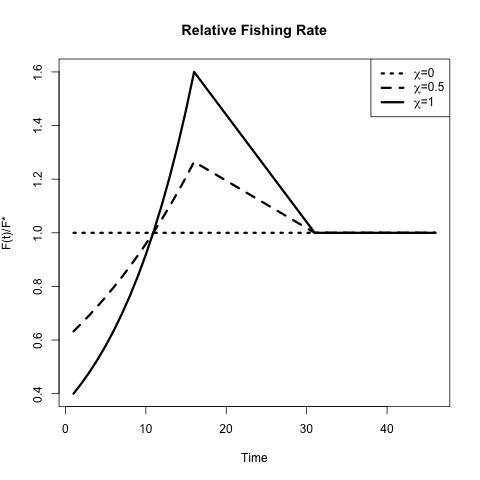
\includegraphics[width=0.44\textwidth]{../ptNew/relFish.png}
$~$
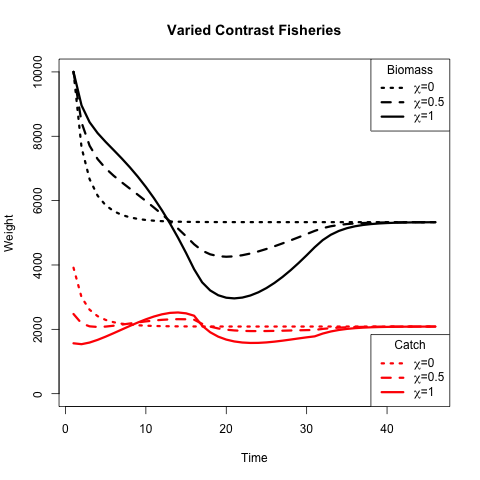
\includegraphics[width=0.44\textwidth]{../ptNew/relSeries.png}
%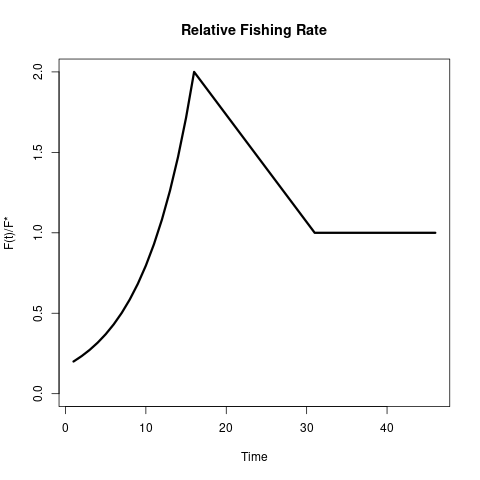
\includegraphics[width=0.45\textwidth]{../../../theses/nick/gpBias/rfExpT45X2Z0.6.png}
%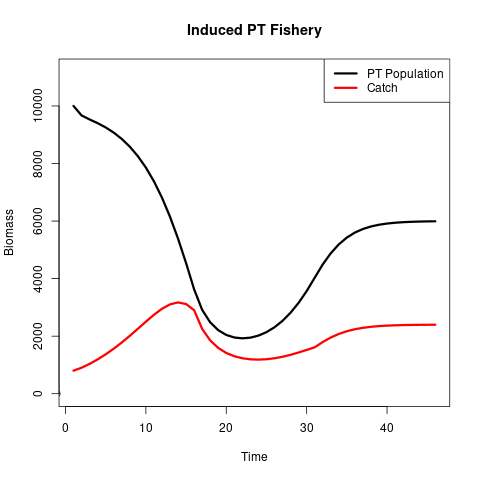
\includegraphics[width=0.45\textwidth]{../../../theses/nick/gpBias/bioCatchExpT45X2Z0.6.png}
%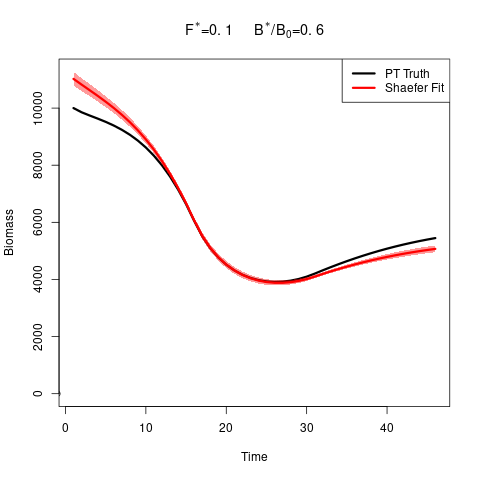
\includegraphics[width=0.5\textwidth]{../../../theses/nick/gpBias/bioPostCompareExpT45X0.5Z0.6.png}
\vspace{-1cm}
\caption{ \label{catchT45}
($left$) Relative fishing with low, medium, and high contrast.
($right$) Population biomass and catch at each associated level of contrast. %demonstrating contrast in a {\color{red}PT population} with $F^*=0.4$ and $\frac{B^*}{\bar B(0)}=0.6$.
}
\label{catch45}
\end{figure}
%\clearpage
%
When $\chi=0$, the relative fishing rate is a constant at 1 to create a low
contrast simulation environment. As $\chi$ increases Eq (\ref{relFish1})
induces more and more contrast in the observed index and catch time series
until $\chi=1$ which produces a high contrast simulation environment.
Figure (\ref{catch45}) demonstrates a spectrum of contrast simulation
environments as well as the time series data they induce in the solution of
the production model ODE.

%\clearpage
\subsection{Two-Parameter Production Model Inference\label{modelFit}}

%
The simulated mapping results from fitting an intentionally misspecified two
parameter production model to index of abundance data that are generated from
a more complex three-parameter model of productivity.
%The simulation results in an intentionally (and controlled) 
%misspecified two-parameter production model. 
%The goal of model fitting is to assess how the biological parameters of the
%two-parameter production model behave under MLE inference when index of 
%abundance data are generated from more complex models of productivity. % three-parameter models, to PT data.
Thus, let $I_t$ be an index of abundance simulated from the three-parameter PT
or Schnute production models at time $t\in\{1,2, 3,..., T\}$. However the
fitted model is specified to be intentionally misspecified so that the fitted
model is driven by a two-parameter Schaefer, or BH production model respectively. %of productivity. 

%
The observation model for the fitted model is log-normal such that,
%
\begin{align}
I_t| q, \sigma^2, \bm{\theta} \sim LN(qB_t(\bm{\theta}), \sigma^2).
\end{align}
%
$B_t(\bm{\theta})$ is defined by the solution of the ODEs defined by the Schaefer, or BH models.
%
For the Schaefer model $\bm{\theta}=[r, K]$, {\color{red}and for the BH model $\bm{\theta}=[\alpha, \beta]$.}
%%
%\begin{align}
%\frac{dB}{dt} = r B \left(1-\frac{B}{K}\right) - FB. \label{odeS}
%\end{align}
%
From the perspective of the fitted model, the observed $I_t$ are assumed independent
conditional on $q$, $\sigma^2$, $r$, $K$ and the two-parameter ODE model for biomass.
Thus the log likelihood can be written as
%
\begin{align}
\log\mathcal{L}(q, \sigma^2, \bm{\theta}; I) = - \frac{T}{2}\log(\sigma^2) - \frac{1}{2\sigma^2}\sum_t \log\left(\frac{I_t}{qB_t(\bm{\theta})}\right)^2. \label{logLike}
\end{align}

%
In this setting, $q$ is fixed at 0.0005 and $M$ is fixed at 0.2, to focus on
the inferential effects of model misspecification on biological parameters.
$\sigma^2$ and $\bm{\theta}$ are reparameterized to the log scale
and fit via MLE.
%$\sigma^2$ is allowed to be fit to assess overall model fit. 
Reparameterizing the parameters to the log scale improves the reliability
of optimization, in addition to facilitating the use of Hessian information
for estimating MLE standard errors.
%$r$ and $K$ are reparameterized as $log(r)$ and $log(K)$ to improve the regularity of 

%
Given that the biological parameters enter the likelihood via a nonlinear ODE,
and further the parameters themselves are related to each other nonlinearly,
the likelihood function can often be difficult to optimize. A hybrid optimization
scheme is used to maximize the log likelihood to ensure that a global MLE solution
is found. The R package GA \cite{scrucca_ga_2013, scrucca_extensions_2017} is
used to run a genetic algorithm to explore parameter space globally.
Optimization periodically jumps into the L-BFGS-B local optimizer to refine
optima within a local mode. The scheme functions by searching globally, with the genetic
algorithm, across many initial values for starting the local gradient-based optimizer.
The genetic algorithm serves to iteratively improve hot starts for the local
gradient-based optimizer. Additionally, optimization is only considered to be converged
when the optimum results in an invertible Hessian at the found MLE.

%
%\clearpage
\subsection{Continuous model formulation}

%
An important (and often overlooked) implementation detail is the solution to the
ODE which defines the progression of biomass through time. % (See Eq(\ref{ode})). 
As a statistical model it is of paramount importance that this ODE not only have a
solution, but also that the solution be unique. Of primary concern, uniqueness
of the ODE solution is necessary for well conditioned inference. %of identifiability of the statistical model.

%
If the form of $\frac{dB}{dt}$ is at least Lipschitz continuous, then the
Cauchy-Lipschitz-Picard theorem provides local existence and uniqueness of
$B(t)$. %, on the condition that the form of $\frac{dB}{dt}$ is at least Lipschitz continuous
Recall from Eq(\ref{ode}) that $\frac{dB}{dt}$ is separated into
a term for biomass production, $P(B)$, and a term for removals, $Z(t)B(t)$.
For determining Lipschitz continuity of $\frac{dB}{dt}$,
the smallest Lipschitz constant of $\frac{dB}{dt}$ will be the sum of the
constants for each of the terms $P(B)$ and $Z(t)B(t)$ separately. Typically any
choice of $P(B)$ will be continuously differentiable, which implies Lipschitz
continuity. % (since the set of continuous differentiable functions is a subset of the set of Lipschitz continuous functions).
At a minimum $Z(t)$ typically contains fishing mortality as a function of time
$F(t)$ to model catch in time as $C(t)=F(t)B(t)$. $Z(t)$ may or may not contain
$M$, but typically $M$ is modeled as stationary in time and does not pose a
continuity issue, unlike some potential assumptions for $C(t)$.
%However, $Z(t)$ typically models fishing mortality as a function of time which . 
%(by more strict definition of continuity than Lipschitz continuity, and furthermore cont
%Thus, the assumed form of $P(B)$ does not typically introduce continuity concerns,
%unlike some potential assumptions for $Z(t)B(t)$.

%
In practice $C(t)$ is determined by a series of observed, assumed known, catches.
Catch observations are typically observed on a quarterly basis, but
in practice may not be complete for every quarter (or year) of the modeled
period. It is overwhelmingly common to discretize the ODE in time via Euler's
method with integration step sizes to match the observation frequency of the
modeled data. This is often computationally convenient when the underlying species
dynamics are resonably well behaved, however when the dynamics model is used
as a statistical model, with the goal of inferring the behavior of the
underlying species dynamics, the regularity of the dynamics are not guaranteed.
%general evaluating  can present several issues. 
%strategy often pushes the assumption of catch continuity under the rug. However, 
An implicit assumption of continuity of catch in time provides the neccessary
regularity for the statistical model. Furthermore a continuous handling of the
dynamics provides improved accruacy in evaluating the ODE, particually when
inferring productivity parameters which largely control the regularity of the
dynamics.

%
While there are many ways to handle catch continuity, here I assume that catches 
accrue linearly between observed catches. This assumption defines the catch
function as a piecewise linear function of time, with the smallest Lipschitz
constant for the catch term defined by the steepest time segment of the catch
function. This assumption represents one of the simplest ways of handling catch,
while retaining Lipschitz continuity overall. Furthermore linearly interpolated
catch is adequately parsimonious for the typical handling of catches.

%
\subsubsection{Integration and Stiffness}

%
As previously mentioned, the overwhelming majority of implementations of
stock assessment models discretized the ODE using Euler's method with the
integration step sized fixed so as to match the observation frequency. In this
setting we explore model parameterizations that explore the full extent of
biologically relevant reference points. This exercise produces some
combinations of parameters that result in numerically stiff ODEs.

%
The concept of stiffness in ODEs is hard to precisely characterize.
%({\color{red}cite}). Hairer and Wanner [5, p. 2] 
Hairer and Wanner \cite[p.2]{wanner_solving_1996} describe stiffness in the
following pragmatic sense, ``Stiff equations are problems for which explicit
methods don't work''. It is hard to make this definition more mathematically
precise, but this a consistent issue for models of very productive species in
the low contrast simulation. 
% parameterized
%so that $\zeta$ is greater than about $\frac{1}{2}$. 
Euler's method, as often implemented, is particularly poorly suited for these
stiff regions of parameter space. In these stiff regions it is necessary to
integrate the ODE with an implicit integration method.

%
Several of the most common implicit methods were tried including the
Livermore Solver for ODEs (lsode), and the Variable Coefficient ODE Solver
(vode) as implemented in the deSolve package of R \cite{soetaert_solving_2010}.
The difference between implicit solvers is negligible, while explicit
methods result in wildly varying solutions to the ODE in stiff regions of
parameter space. %explicate methods completely fail to represent the model as
%stated in the stiff regions of parameter space. 
Results shown here are computed using the lsode integration %method 
since it runs relatively quickly and has a relatively smaller footprint in system memory.

%Too stiff for Euler,
%avoid chaos, and
%implicit methods

%
%RESULTS
%

%
\clearpage

%\vspace*{-1.5cm}
\section{Results}

%
\subsection{An $MSY$-Optimal Catch History \label{flat}}

%
When $F(t)$ is held constant at $F^*$, as it is in the ``low contrast''
simulation setting, $B(t)$ comes to equilibrium as an exponential decay from
$K$ to $B^*$. Understanding model misspecification bias is simplified in this
setting due to the relative simplicity that this induces in $B(t)$. However
this simplicity is known to poorly inform estimates of $r$, and thus $F^*$,
due to the limited range of the production function that is observed
\cite{hilborn_quantitative_1992}.
%This example is a "low contrast" setting.

%%
%Figure (\ref{flatProd}) shows four of the most misspecified example Schaefer 
%function fits as compared to the true data generating PT production
%functions. In the rug plots below each set of curves the observed biomasses
%demonstrate the exponential decay from $K$ to $B^*$ in each case. In particular,
%notice how only biomasses greater than the PT $B^*$ are observed. 
%Due to the
%leaning of the true PT curves, and the symmetry of the logistic parabola, the
%logistic curve only observes information about its slope at the origin from
%data observed on the right portion of the PT curves. Above the Schaefer line
%PT is steeper on the right of $B^*$ than it is on the left, and so the the
%logistic curve over-estimates $r$, and thus $F^*$, for data generated above
%the Schaefer line. Below the Schaefer line the vice versa phenomena occurs.
%Below the Schaefer line PT is shallower to the right of $B^*$ than it is on the
%left and so the logistic parabola estimate tends to under estimate $F^*$.

%\begin{figure}[h!]
\begin{wrapfigure}{r}{0.5\textwidth}
\vspace{-0.5cm}
%\begin{minipage}[h!]{0.49\textwidth}
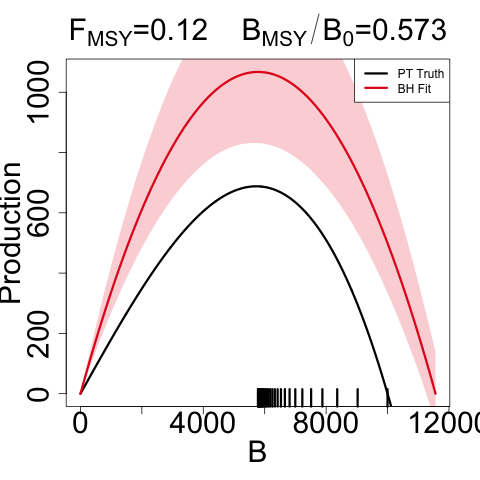
\includegraphics[width=0.24\textwidth]{../ptNew/srrCompareFlatT30X0.12Z0.573.png}
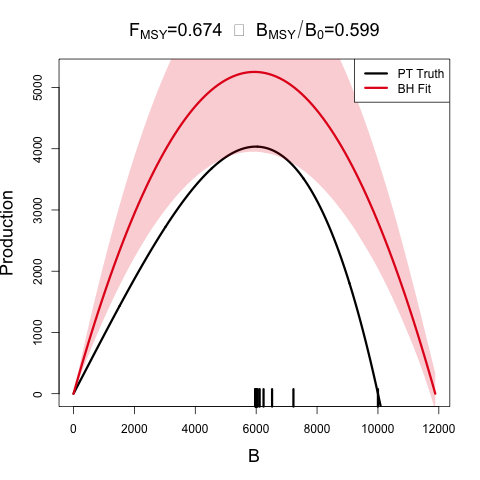
\includegraphics[width=0.24\textwidth]{../ptNew/srrCompareFlatT30X0.674Z0.599.png}\\
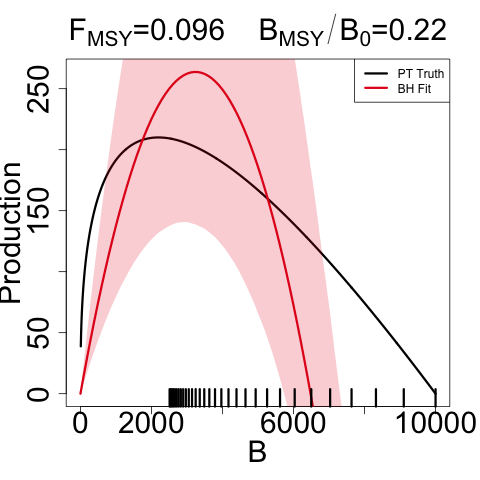
\includegraphics[width=0.24\textwidth]{../ptNew/srrCompareFlatT30X0.096Z0.22.png}
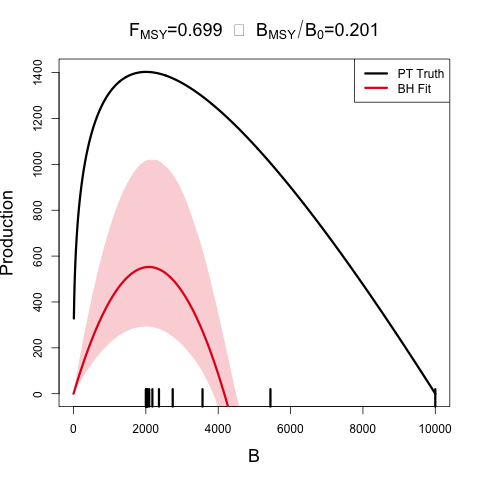
\includegraphics[width=0.24\textwidth]{../ptNew/srrCompareFlatT30X0.699Z0.201.png}
%\end{minipage}
%\begin{minipage}[h!]{0.49\textwidth}
%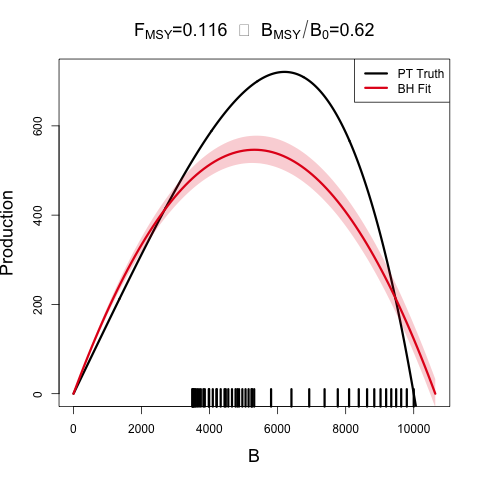
\includegraphics[width=0.45\textwidth]{../ptNew/srrCompareExpT45X0.116Z0.62.png}
%%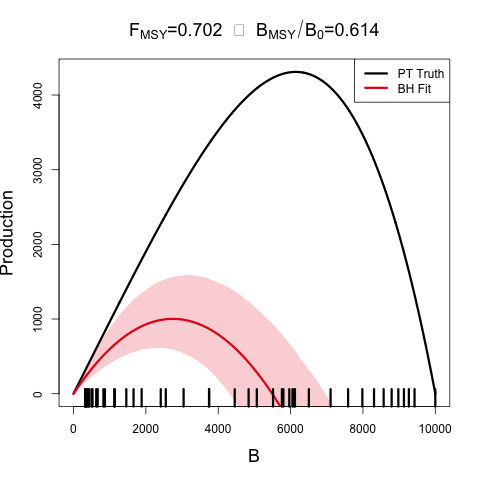
\includegraphics[width=0.45\textwidth]{../ptNew/srrCompareExpT45X0.702Z0.614.png}\\
%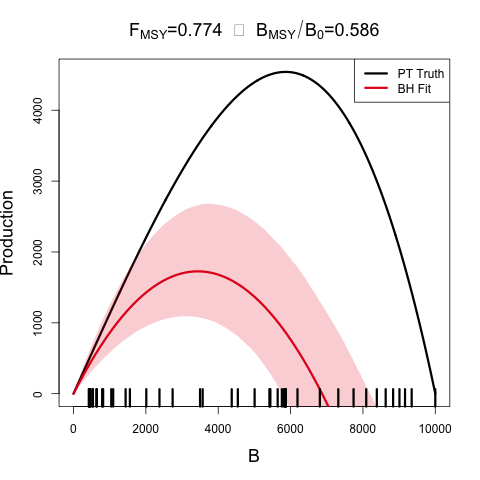
\includegraphics[width=0.45\textwidth]{../ptNew/srrCompareExpT45X0.774Z0.586.png}\\
%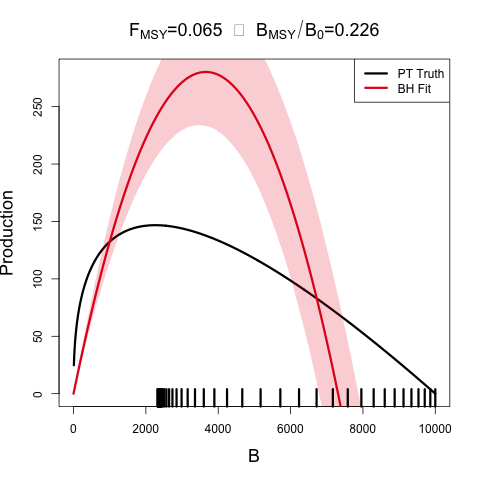
\includegraphics[width=0.45\textwidth]{../ptNew/srrCompareExpT45X0.065Z0.226.png}
%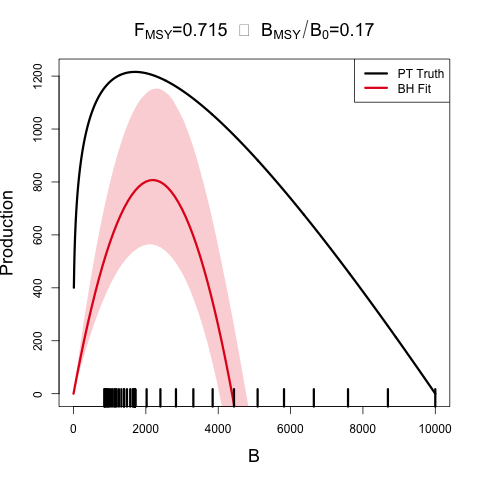
\includegraphics[width=0.45\textwidth]{../ptNew/srrCompareExpT45X0.715Z0.17.png}
%\end{minipage}
\caption{
A comparison of the true PT production function (in black) and the estimated logistic curve (in red)
with 95\% CI shown. The examples shown represent the four corners of maximum model misspecification
in the simulated RP-space. Observed biomasses are plotted in the rug plots below the curves.
%Fitted logistic production function verses true PT production function. 
%Observed biomass plotted along x-axis.
}
\label{flatProd}
%\end{figure}
\end{wrapfigure}

%
Figure (\ref{flatProd}) shows four of the most misspecified example
production function fits as compared to the true data generating PT production
functions. The rug plots below each set of curves show how the observed
biomasses decay exponentially from $K$ to $B^*$ in each case. In particular,
notice how observations only exist where the PT biomass is greater than $B^*$.
Due to the leaning of the true PT curves, and the symmetry of the logistic
parabola, the logistic curve only observes information about its slope at the
origin from data observed on the right portion of the PT curves. The top two
panels of Figure (\ref{flatProd}) shows PT data generated such
that $\frac{B^*}{\bar B(0)}>0.5$; in these cases PT is steeper to the right of
$B^*$ than it is on the left, and so the the logistic curve over-estimates $r$,
and consequently also over-estimates $F^*$. %for data generated above the Schaefer line. 
The bottom two panels of Figure (\ref{flatProd}) show PT data
generated with $\frac{B^*}{\bar B(0)}<0.5$ and where the vice versa phenomena
occurs. PT is shallower to the right of $B^*$ than it is on the left and so the
logistic parabola estimate tends to under estimate $F^*$.

%
\subsubsection{Metamodeled Trends}

%\item define Schaefer line.
%\item reiterate each point in RP space is an entire PT model, on the Schaefer 
%line moder are Schaefer.

%
Each point in the space of the RPs $F^*$ and $\frac{B^*}{\bar B(0)}$ uniquely
identifies a complete PT model with different combinations of parameters values.
Recall that when $\gamma=2$ for the PT model, the PT curve becomes a parabola
and is equivalent to the logistic curve of the Schaefer model. Since the
logistic curve is symmetric about $B^*$, the Schaefer model must fix the value of
$\frac{B^*}{\bar B(0)}$ at the constant $0.5$ for any value of $F^*$. So
the line through RP space defined by $\frac{B^*}{\bar B(0)}=0.5 ~~ \forall ~~ F^*$,
defines the subset of RP space where $\gamma=2$ and where the PT model is
equivalent to the Schaefer model. For brevity this subset of RP where $\frac{B^*}{\bar B(0)}=0.5$
will be referred to as the ``Schaefer set''. Thus simulated data that are
generated along the Schaefer set will be the only data that are not
misspecified relative to the Schaefer model; as PT data are simulated
farther and farther away from this line at $\frac{B^*}{\bar B(0)}=0.5$ model
misspecification of the Schaefer model becomes worse and worse.

%\item generalize the srr figure above
%\item individual model fits will have jittery trends; metamodel nonlinearly 
%smooths and pulls information together.

%
While Figure (\ref{flatProd}) demonstrates a real trend in simulation results,
individual simulation runs will at best show jittery trends due to the stochastic
nature of statistical inference. The GP process metamodel accounts for this
stochasticity %, filters out jitters, %  and allows for the jitters to be filtered out 
to focus analysis on the signal in the simulation results. Recall that metamodeling
occurs on the scale of the inferred productivity parameters of the restricted
production model,
%by transforming  %(in this case the Schaefer model when fitting PT data. 
by transforming metamodel predictions via Eq. (\ref{ptRP}), metamodeled predictions
are obtained for Schaefer RPs. By further subtracting the true data generating
PT RPs from the predicted Schaefer RPs at each point in RP space a pattern of
inferential RP bias, induced by model misspecification of the Schaefer model,
can be seen. %to be seen. % in Figure (\ref{arrowsPT}).

%using the relevant transformations given in Eq. (\ref{ptRP}) , \ref{BratS}, \ref{FmsyS}) with $\gamma$
%fixed to the restricting case.
%
%Additionally the metamodel generalizes the patterns seen in Figure (\ref{flatProd}) across the entire range of RPs. 

%../ptNew/ptLook.r
\begin{figure}[h!]
\begin{minipage}[h!]{0.44\textwidth}
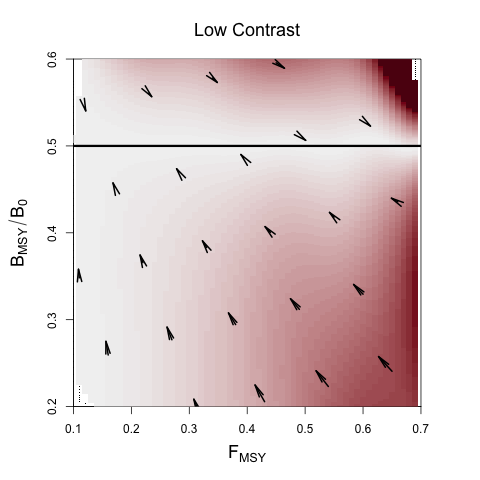
\includegraphics[width=\textwidth]{../ptNew/directionalBiasSubPTFlatT30.png}
\end{minipage}
\begin{minipage}[h!]{0.44\textwidth}
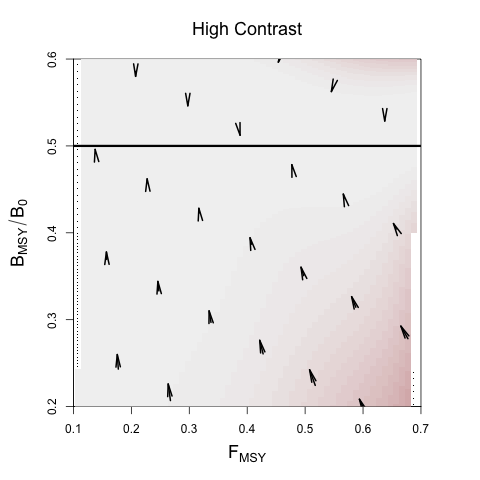
\includegraphics[width=\textwidth]{../ptNew/directionalBiasSubPTExpT45MinCon.png}
\end{minipage}
\begin{minipage}[h!]{0.09\textwidth}
\hspace{-1cm}
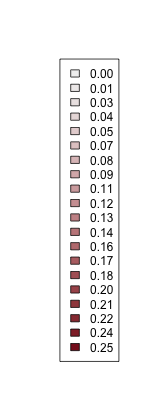
\includegraphics[width=1.5\textwidth]{../ptNew/subLegnd.png}
\end{minipage}
\caption{
Joint bias direction for ($F^*$, $\frac{B^*}{B_0}$) estimates under
the misspecified Schaefer Model. The intensity of color represents the excess
bias relative to the shortest possible mapping. Results in the low contrast setting
are shown $left$, and the high contrast setting is shown $right$.
}
\label{arrowsPT}
\end{figure}

%
Figure (\ref{arrowsPT}) shows the pattern of biases the Schaefer model creates when fit
to PT data generated at each point of RP space. An equivalent way to think of Figure
(\ref{arrowsPT}) is that since the Schaefer model must estimate RPs in the Schaefer set,
the metamodel arrows indicate the mapping that is created by inferring RPs under
a misspecified Schaefer model fit to PT data generated at each point over the pictured
region.

%
Since $\frac{B^*}{B_0}$ must be 0.5 under the Schaefer model, biases in the
$\frac{B^*}{B_0}$ direction must simply map vertically onto the Schaefer set.
Due to this simplified RP geometry under the Schaefer model, the degree of bias in
$\frac{B^*}{B_0}$ estimation is defined solely by the degree of model
misspecification irrespective of $F^*$. Furthermore,
%since the Schaefer line is simply a constant at $\frac{B^*}{B_0}=0.5$, 
the closest possible point along the Schaefer set that Schaefer model inference %under a Schaefer model 
could map RPs would be the perfectly vertical mapping. This pattern only contains the
strictly necessary bias present in $\frac{B^*}{B_0}$, and zero bias in $F^*$.
Any deviation from this minimal bias pattern is necessarily due to added bias in $F^*$.

%
The two simulation settings shown in Figure (\ref{arrowsPT}) are identical except
for the amount of contrast present in the simulated index. The left panel of
Figure (\ref{arrowsPT}) shows RP biases in the low contrast setting, while the
right panel shows the high contrast setting. Notice that in the low contrast
setting the RP bias pattern is far from the minimum distance mapping, however when
contrast is added the mapping becomes much closer to a minimal vertical bias mapping.
In the low contrast setting the observed bias is consistent with the pattern
and mechanism described in Figure (\ref{flatProd}), where $F^*$ is underestimated
for data generated below the Schaefer line and overestimated above the Schaefer set.
In the high contrast simulation the mapping is nearly minimal distance with the exception
of PT data generated with simultaneously low $\frac{B^*}{B_0}$ and high $F^*$.

%
%\begin{wrapfigure}{r}{0.5\textwidth}
%\vspace{-0.5cm}
\begin{figure}
\begin{minipage}[h!]{0.49\textwidth}
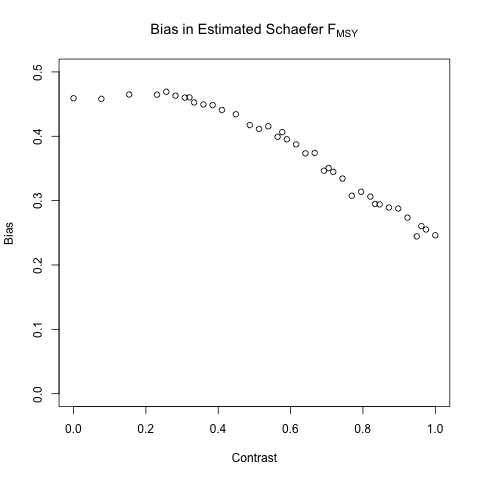
\includegraphics[width=\textwidth]{../ptNew/contrastTest.png}
\end{minipage}
\begin{minipage}[h!]{0.49\textwidth}
\caption{
Bias in $F^*$ under the Schaefer model when PT data are generated
with increasing contrast so that $F^*$ and $\frac{B^*}{B_0}$ are fixed at
0.699 and 0.201 respectively. %Bias is shown for the Schaefer models estimation of $F^*$ as a function of contrast.
%A comparison of the true PT production function (in black) and the estimated logistic curve (in red)
%with 95\% CI shown. The examples shown represent the four corners of maximum model misspecification
%in the simulated RP-space. Observed biomasses are plotted in the rug plots below the curves.
%%Fitted logistic production function verses true PT production function. 
%%Observed biomass plotted along x-axis.
}\label{conTest}
\end{minipage}
\end{figure}
%\end{wrapfigure}

%
Figure (\ref{conTest}) demonstrates how bias in $F^*$ estimation %under the Schaefer model 
decreases as contrast is added to PT data as generated in the low $\frac{B^*}{B_0}$ and
high $F^*$ regime. By including additional contrast $F^*$ bias is decreased, however
parameterizing contrast so as to fully extinguish $F^*$ bias may require a more complex
model of fishing.
%,  in may be By including more contrast $F^*$ bias  in this low $\frac{B^*}{B_0}$, 
%high $F^*$ region can be further reduce.}

%
\section{Discussion}

%;
%the simulation design and metamodeling methods presented here further generalize these
%results of these existing results.
%Existing

{\color{blue} {\it Tease Out BH}\\

%
Results presented here generally agree with what is known about estimating population
growth rate parameters \cite{lee_can_2012, conn_when_2010, magnusson_what_2007}.
These studyies appreciate the role of contrast for estimating growth rates,
however they struggle to make generally extensible conclusions since they focus only
on a handful of stocks that fall short of forming a random sample of the greater
population of possible stock behaviors. The LHS design methods presented here are
designed specifically to simulate a representative sample of stocks broadly
across the space of possible RPs. Furthermore, the simulation design, taken together
with the GP metamodel of productivity parmater estimates, allows this study to control
the degree of model misspecification and generalize conclusions about the behavior
of productivity estimation within the production model setting presented.

%%
%Unfortunately, we are unable to generalize the relationship because the twelve 
%assessment examples are not a random sample from the population of all fish 
%stocks and sample size is small. A more general conclusion may be obtained by 
%including more assessments
%%
%\begin{itemize}
%\item \shortcite{lee_can_2012} Generalizability via random sample of fisheries, LHS RP explicitly does this.
%\item multiple starting locations and convergence defined as positive definite Hessian.
%\end{itemize}

%
In the presence of contrast, $F^*$ estimation can enjoy very low bias even
for a wide range of poorly specified models; conversely in the absence of contrast
$F^*$ estimation can suffer very large bias even for slightly misspecified models.
This pattern is particularly true for low-contrast inference under the Schaefer model where the
geometry of the restricted RP set isolates estimation failure of $F^*$ from
$\frac{B^*}{\bar B(0)}$. While contrast has a similar impact on $F^*$ estimation
under the BH model, the geometry of the BH RP set correlates estimation bias
of $F^*$ and $\frac{B^*}{\bar B(0)}$. The GP metamodeling approach reveals a
more general pattern that highly informative data sets (high contrast)
produces a nearly minimal distance mapping of RPs %that are nearly minimal distance mapping 
onto the constrained RP set.

%
In all cases when model misspecification is removed, even with weakly informative
data, RP estimation is unbiased and well estimated. Thus contrast alone is
not the only factor leading to inferential failure. Model misspecification is a
necessary but not sufficient condition for inducing RP estimation bias. The
particular RP bias present depends on the RP geometry of the fitted model and
how that geometry is misspecified relative to the data. The RP mapping is then oriented
to the RP geometry of the fitted model.

%
%NOTE: BITCH ABOUT NOT BEING ABLE TO PRODUCE A PERFECTLY INFORMATIVE TIME SERIES
%SPECULATE ABOUT IDEALLY INFORMATION CATCH PATTERNS (DYNAMIC CALIBRATION OF $F^*$)
While the relative fishing rate parameterized in Section (\ref{catch}) captures a usefully
broad spectrum of relevant fishing behaviors, it is still limiting in the amount of information
that it can induce. Improved methods for quantifying contrast in fisheries data, and/or methods of
discovering more informative fishing behavior, could improve this analysis. In the absence of a %Without knowing a 
maximally informative dataset simulation methods will not fully describe how
inference fails, but the methods presented here tell the most complete picture
yet, with explicit control of the degree model misspecification, contrast, and
a simulation design that allows for uniform representative data generation
across biologically meaningful stocks. The results presented here suggest the
conjecture that under a maximally informative dataset, RP inference with a two
parameter production function will be biased in the direction a shortest distance
map from the true RPs onto restricted set of RPs under the two-parameter model.

%
Given the potential for model misspecification of RPs, a minimal distance
mapping of RPs represents a best-case scenario where the total bias of RPs,
when measured jointly, is minimized. That said, without recognizing the
geometry of how two-parameter models of productivity limit RP space this may
lead to unintuitive implications in RP estimation. For example, due to the
shape of the BH RP set a minimal distance mapping ensures that if there is
bias in one of $\frac{B^*}{B_0}$ or $F^*$, there will necessarily be
bias in the other RP. However under the Schaefer model, since the RP set is a
constant in $\frac{B^*}{B_0}$, bias in $F^*$ is not adulterated in the
same way by bias in $\frac{B^*}{B_0}$ estimation. While models with
constant RPs, such as the logistic model $\frac{B^*}{B_0}=\frac{1}{2}$ or
the Fox model $\frac{B^*}{B_0}=\frac{1}{e}$, are extremely limited, they
can be valuable tools for developing intuition precisely because they isolate
RP estimation in their free RPs from the correlated RP biases present in
models like the BH or Ricker model.

%
When one considers the implications of RP bias, overestimation of RPs carries
the severe implication of management recommendations potentially leading to
overfishing, while underestimation of RP leads to overly conservative management.
In this sense, when the true model is not known, the geometry of the BH set together
with the metamodeled bias trends makes the BH model a naturally conservative
estimator of RPs for most stocks. For most non-BH populations the BH model is
likely to make conservative errors in its estimates of $F^*$ and $\frac{B^*}{B_0}$.
The one notable exception to the conservatism of the BH model stands for data
generated in the Cushing-like regime of Schnute RPs. In this regime the BH
model tends to be fairly unbiased overall, however the bias that is present
for these populations tends to be overestimation in both RPs, leading to much
more severe management consequences for those populations.

%
The RP bias trends of the Schaefer model demonstrate much less {\color{red}conservatism} than the BH overall.
For any population with $\frac{B^*}{B_0}<0.5$, $\frac{B^*}{B_0}$ will be overestimated.
When the population comes from the regime where $\frac{B^*}{B_0}>0.5$, $\frac{B^*}{B_0}$
will be under estimated, but $F^*$ is likely to be overestimated depending on the degree of
contrast present in the data. So while the Schaefer model is an intuitive model, it tends to
lead to much less conservative RP estimation.

%
While it is important to recognize these limitations of two-parameter models
of productivity, we should not solely accept conservativism as a rational of
choosing a BH model of productivity. %Ultimately accuracy of RP estimation, 
%without structural RP biases, %and accurate assessment of uncertainty is a better state 
Increasing the flexibility of the production function by moving toward
three-parameter models would release the underlying structural limitations
\cite{mangel_perspective_2013} that cause these RP biases in the first place.
Punt \& Cope \cite{punt_extending_2019} %(Mangel et al., 2013). Punt and Cope (2019) 
considers a suite of possible three-parameter curves which could be used
instead of current two-parameter curves. For all of their benefits, three
parameter production functions have their own complicating factors, and the
structure present in the Schnute model explored here makes it an intuitive bridge
model for developing three-parameter models going forward.

}





